\documentclass[main.tex]{subfiles}
\begin{document}
\begin{titlingpage}
\begin{center}

~ \\[3cm]

%\includegraphics[width=0.6\textwidth]{figurer/ASE}~\\[1cm]

\textsc{\LARGE Bilag 2}\\[1.5cm]

%\textsc{\Large Sundhedsteknologi}\\
%\textsc{\Large 3. semesterprojekt}\\[0.5cm]

\noindent\makebox[\linewidth]{\rule{\textwidth}{0.4pt}}\\
[0.5cm]{\Huge Analyse}
\noindent\makebox[\linewidth]{\rule{\textwidth}{0.4pt}}
\end{center}
\vfill
\begin{center}
{\large 19. december 2017}
\end{center}
\end{titlingpage}

\newpage
\tableofcontents*
\newpage

\chapter{Indledning}


I afsnittet analyse vil der blive beskrevet de overvejelser om mulige løsninger i projektet og hvilke der har valgt at gå videre og begrundelse herom. Der er beskrevet og diskuteret valget af hardware- og software komponenter som er kritiske for systemet. Det udleveret diagram som kan ses på figur \ref{BIdiagram} blev realiseret som det første ved analysen, for at sikre at det vil kunne bruges senere i arkitekturen og implementering. Dette er en simple BI måler som består af en instrumenterings forstærker, en strømgenerator og udgang til elektroder. Kredsløbet skal tilføres et signal fra en funktion generator, som resulterer i en konstant genereret strøm over elektroderne. Da man nu har en kendte strøm og måler spændingsfaldet over elektroderne, kan man ved brug af ohms lov (U/I=R) beregne impedansen for et synk.


\begin{figure}[H]
\centering
{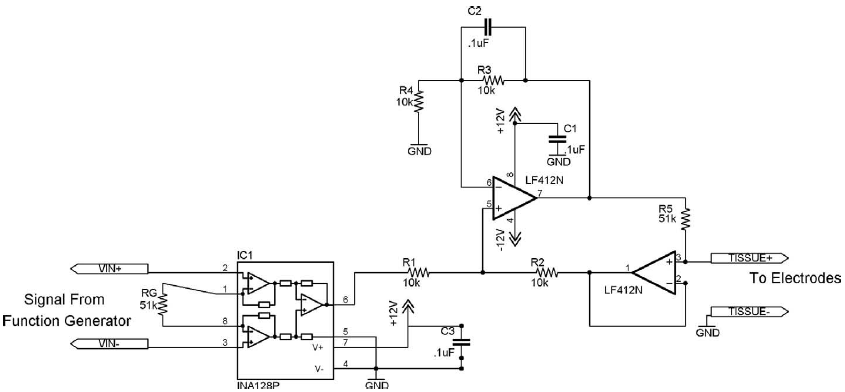
\includegraphics[width=\linewidth]
{Figure/BIdiagram}}
\caption{BI diagram\cite{Aroom2009}}
\label{BIdiagram}
\end{figure}



\chapter{Hardware}
\section{Bioimpedans}



\begin{figure}[H]
\centering
{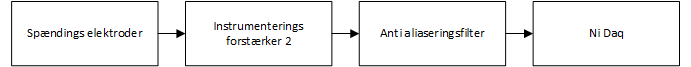
\includegraphics[width=\linewidth]
{Figure/analyse2}}
\caption{Bioimpedans ind}
\label{BIdiagram}
\end{figure}

\subsection{Analyse af kristiske komponenter til BI}

\begin{figure}[H]
\centering
{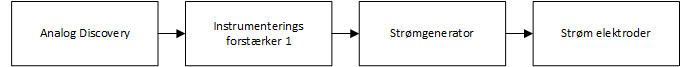
\includegraphics[width=\linewidth]
{Figure/analyse1}}
\caption{Bioimpedans ud}
\label{BIdiagram}
\end{figure}

\subsubsection{Instrumenterings forstærker 1}
I det oprindelig design af BI konstateret vi at det var lavet lavet til at måle BI'er på skalpen og ikke over svælget. Derfor valgte vi at instrumenterings forstærkeren fik et større signal ind fra Analog Discovery på 2V og 50kHz. I det hele taget undrede vi over artiklens valg af brug af instrumenterings forstærker i starten af kredsløbet, da den ikke er et must for at realisere kredsløbet. Men dens eneste formål var at nedbringe common-mode støj fra funktions generatoren, så vi valgte at beholde denne da vi også vil undgå så meget støj som muligt videre i kredsløbet. Gain var oprindeligt sat til 51 Kohm hvilket giver det dobbelte af hvad instrumenterings forstærkeren tilføre. I diagrammet på figur \ref{BIdiagram} kan det ses at instrumenterings forstærkeren bliver forsynet med +12/-12 V, men der er her valgt at -12 V skal direkte til ground, hvilket har resulteret i at instrumenterings forstærkeren ikke fungerer korrekt, så der er den i stedet forsynet med -12 V og ikke ground.  





\subsubsection{Strømgenerator}
Det forstærket signal som kommer fra udgangen på instrumenterings forstærkeren løber over til strømgeneratoren. Denne strømgenerator er en Howland bridge. Sammensætningen af modstandene er vigtige og deres tolerance skal være lav for at få en korrekt og konstant strøm. For at justerer strømmen kan R5 udskiftes i kredsløbet. For at få en konstant strøm omkring ca. 500 uA, er modstanden ændret fra 51 Kohm til 2 Kohm.  

\begin{center}
  \begin{tabular}{ r |  r }
    \hline
    Hz & uA \\ \hline
    100 & 49 \\ \hline
    200 & 40 \\ \hline
    300 & 35 \\ \hline
    400 & 32 \\ \hline
    500 & 30 \\ \hline
    600 & 29 \\ \hline
    700 & 28 \\ \hline
    800 & 27 \\ \hline
    900 & 27 \\ \hline
    1000 & 27 \\ \hline
    2000 & 24 \\ \hline
    3000 & 21 \\ \hline
    4000 & 19 \\ \hline
    5000 & 17 \\ \hline
    6000 & 14 \\ \hline
    7000 & 12 \\ \hline
    8000 & 10 \\ \hline
    9000 & 7 \\ \hline
    10000 & 5 \\ \hline
    20000 & 0 \\ \hline
    
    
  \end{tabular}
\end{center}















\begin{figure}[H]
\centering
{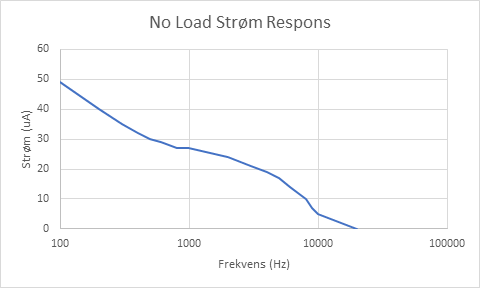
\includegraphics[width=12cm]
{Figure/stromfrekvensoprindelig}}
\caption{No load strøm respons af det konstante strømkredsløb VCCS. }
\label{stromfrekvens}
\end{figure}



\section{AD konverter}
\section{Overvejelser om mulige løsninger}
\section{løsninger I har valgt, begrundelsen herfor}
\section{grundlæggende valg af hardware- og softwaremæssige komponenter, som er kritiske for realisering af systemet}

\section{For at træffe et valg kan der analyseres og diskuteres forskellige løsninger mht. til ydeev-ne, pris, leveringstid og forhåndskendskab. Disse kan med fordel opstilles i tabelform.}

\subsection{Anti-alisering}
\section{Elektroder}
\section{EMG}
\section{Analog Discovery}
\section{Testopstillinger}
\subsection{Konstant strøm}
\subsection{Lavpas filtering}
\subsection{Ensretter}
\subsection{Sampling af signal}




\chapter{Software}
\section{Waveforms}
\section{Matlab}

\chapter{Konklusion}

\bibliography{Mendeley.bib}
\end{document}


